\documentclass[10pt,openright,twoside,french]{book}

\input philippe2013
\input philippe2013_cours
\input philippe2013_sections
\input philippe2013_chapitre
\renewcommand\PartProgramme{Géométrie}
\renewcommand\MaCouleur{Purple}

\pieddepage{}{%
\begin{tikzpicture}[scale=0.65]
\shadedraw [top color=white, bottom color=\MaCouleur, draw=\MaCouleur]
[l-system={Sierpinski triangle, step=1pt, angle=60, axiom=F, order=6.5}]
lindenmayer system -- cycle;
\draw (30:0.65cm) node {\bfseries\textcolor{black}{\thepage}};
\end{tikzpicture}%
}{}


\setcounter{chapter}{3}
\begin{document}
\chapter[Nombres complexes : forme algébrique]{Nombres complexes\\ Forme algébrique}\label{complexe_algebrique}

\section{Ensemble $\C$}

\begin{Defi}
    Le nombre \iptb{$\I$}\index{i@\I} est le nombre tel que $\I^2 = -1$.
\end{Defi}

\begin{Rmq}
    Le nombre $\I$ n'est pas un nombre réel puisque son carré est négatif.
\end{Rmq}

\begin{Defi}
    On appelle \iptb{nombre complexe}\index{nombre!complexe}\index{complexe} tout nombre $z$ pouvant s'écrire sous la forme $z = x + y\I$, où $x$ et $y$ sont deux nombres réels quelconques.\par
    Cette écriture est la \iptb{forme algébrique}\index{forme!algébrique} du nombre $z$.\par
    $x$ est appelé la \iptb{partie réelle}\index{partie!réelle} de $z$ et se note $x = \Re(z)$.\par
    $y$ est appelé la \iptb{partie imaginaire}\index{partie!imaginaire} de $z$ et se note $y = \Im(z)$.\par
\end{Defi}

\begin{Exemple}[s]
    $a = 4 + 2\I$ est un nombre complexe : $\Re(a) = 4$ et $\Im(a) = 2$.\par\medskip
    $b = -1 + 3\I$ est un nombre complexe : $\Re(b) = -1$ et $\Im(b) = 3$.\par\medskip
    $c = \frac{6 - 3\I}{2}$ est un nombre complexe : $\Re(c) = \frac 6 2 = 3$ et $\Im(c) = \frac{-3}{2}$.\par\medskip
    $d = \sqrt 2 + \sqrt 5 \,\I$ est un nombre complexe : $\Re(d) = \sqrt 2$ et $\Im(d) = \sqrt 5$.\par\medskip
    $e = \I$ est un nombre complexe : $\Re(e) = 0$ et $\Im(e) = 1$.
\end{Exemple}

\begin{Defi}
    On appelle \iptb{$\C$}\index{C@$\C$} l'ensemble des nombres complexes.
\end{Defi}

\begin{Prop}
    Tout nombre réel est un nombre complexe.\par
    Par conséquent, l'ensemble des nombres réels est inclus dans l'ensemble des nombres complexes. On a : $\N \subset \Z \subset \Q \subset \R \subset \C.$
\end{Prop}

\begin{Demo}
    Soit $a \in \R$. On peut écrire $a$ sous la forme $a = a + 0 \times \I$ donc $a \in \C$ et $\Re(a) = a$ et $\Im(a) = 0$.
\end{Demo}

\begin{Defi}
    Soit $z = x + y\I$ un nombre complexe.
    \begin{enumerate}
        \item Si $\Im(z) = 0$ alors $z$ est un nombre réel.
        \item Si $\Re(z) = 0$ alors $z$ est un \ipt{imaginaire pur}.
    \end{enumerate}
\end{Defi}

\begin{Exemple}[s]
    \begin{itemize}
        \item Les nombres $\I$, $2\I$, $\frac{-5\I}{7}$ sont imaginaires purs.
        \item Les nombres $3$, $-\sqrt 6$, $\pi$, $0$ sont des réels.
    \end{itemize}
\end{Exemple}

\section{Opérations sur les nombres complexes}
\subsection{Prolongements des opérations de $\R$}

On admet le théorème suivant :

\begin{Thm}
    Les propriétés de calculs valables dans $\R$ restent valables dans $\C$ : associativité, commutativité, distributivité, identités remarquables. En particulier, en notant $z = x+y\I$ et $z' = x' + y'\I$, on a :
    \[\begin{array}{rcl}
        z + z' &=& (x + x') + (y + y')\I \\
        z \times z' &=& (xx' - yy') + (xy' + x'y)\I \\
        1 \times z & = & z \\
        0 + z & = & z \\
        -z &=& -x - y\I
    \end{array}\]
\end{Thm}

\begin{Exemple}[s]
    Soient $z_1 = 3 + 2\I$, $z_2 = 1 - 3\I$ et $z_3 = -4\I$.\par
    Calculer : $z_1 + z_2$ ; $z_2 \times z_3$, $-z_2$, $(z_1 + z_3) \times z_2$.
\end{Exemple}\medskip

On admet également le théorème suivant :

\begin{Thm}
    Soient $z$ et $z'$ deux nombres complexes.
    \[z = z' \quad \Leftrightarrow \quad \left\{\begin{array}{rcl} \Re(z) & = & \Re(z') \\ & \text{\textbf{et}} & \\ \Im(z) & = & \Im(z') \end{array}\right.\]
\end{Thm}

\begin{Rmq}
    En particulier, en posant $z = x + y\I$, on a : $z = 0 \Leftrightarrow (x = 0 \text{ et } y = 0)$.
\end{Rmq}

\begin{Defi}
    Deux nombres complexes non nuls $z$ et $z'$ sont des \iptb{nombres inverses}\index{inverse} lorsque $z \times z' = 1$.\par
    On écrit alors $z' = \frac 1 z$ ou encore $z = \frac{1}{z'}$.
\end{Defi}

\begin{Thm}
    Tout nombre complexe $z = x + y\I$ non nul admet un inverse $z'$ tel que :
    \[z' = \frac 1 z = \frac{x}{x^2 + y^2} - \frac{y}{x^2 + y^2}\I.\]
\end{Thm}

\begin{Demo}
    $\begin{array}[t]{rcl}
        \frac 1 z & = & \frac{1}{x + y\I} \\[9pt]
                      & = & \frac{x - y\I}{(x + y\I)(x - y\I)} \\[9pt]
                      & = & \frac{x - y\I}{x^2 + y^2} \\[9pt]
                      & = & \pfr{\frac{x}{x^2 + y^2} - \frac{y}{x^2 + y^2}\I}
    \end{array}$

    Le théorème est bien démontré.
\end{Demo}

\subsection{Conjugué d'un nombre complexe}

\begin{Defi}
    Soit $z = x + y\I \in \C$. On appelle \iptb{nombre conjugué}\index{nombre!conjugué}\index{conjugué} de $z$ le nombre complexe noté $\overline z$ défini par :
    \[\overline z = x - y\I.\]
\end{Defi}

\begin{Rmq}
    Deux nombres sont conjugués lorsqu'ils ont la même partie réelle et que leur partie imaginaire sont opposés.
\end{Rmq}

\begin{Exemple}[s]
    Déterminer les nombres conjugués des nombres suivants :\par $z_1 = 3 + 2\I$, $z_2 = 1 - 3\I$, $z_3 = -4\I$ et $z_4 = 5$.
\end{Exemple}

\begin{Prop}
    Soit $z \in \C$. $z = \overline z \Leftrightarrow z \in \R$.
\end{Prop}

\begin{Demo}
    Notons $z = x + y\I$.\par
    $\Leftarrow$ : $z \in \R \Rightarrow z = x + 0 \times \I \Rightarrow \overline z = x - 0 \times \I = x = z$.\par\medskip
    $\Rightarrow$ : $z = \overline z \Rightarrow x + y\I = x - y\I \Rightarrow 2y\I = 0 \Rightarrow y\I = 0 \Rightarrow y = 0 \Rightarrow z \in \R$.
\end{Demo}

\begin{Prop}
    Soit $z = x + y\I \in \C$. Alors : $z \times \overline z = x^2 + y^2$.
\end{Prop}

\begin{Demo}
    $z \times \overline z = (x + y\I)(x - y\I) = x^2 - xy\I + xy\I -y^2\I^2 = x^2 + y^2$.
\end{Demo}

\begin{Prop}
    Pour tous nombres complexes $z$ et $z'$ :
    \begin{enumerate}
        \item $\overline{z + z'} = \overline z + \overline{z'}$.
        \item $\overline{z \times z'} = \overline z \times \overline{z'}$.
        \item Si $z \neq 0$, $\overline{\left(\frac{z}{z'}\right)} = \frac{\overline z}{\overline{z'}}$.
    \end{enumerate}
\end{Prop}

\begin{Demo}
    Démontrons par exemple le deuxième point.\par
    On note $z = x + y\I$ et $z=x' + y'\I$. On effectue les calculs séparément.\par
    $z \times z' = (x + y\I)(x' + y'\I) = xx' - yy' + (xy' + x'y)\I$ donc :\par
    $\overline{z \times z'} = \pfr{xx' - yy' - (xy' + x'y)\I}$.\par\medskip
    $\overline z \times \overline{z'} = (x - y\I)(x' - y'\I) = xx' - xy'\I - x'y\I + yy'\I^2 = \pfr{xx' - yy' - (xy' + x'y)\I}$.
\end{Demo}

\section{Représentation géométrique}

On muni le plan $\calig P$ d'un repère orthonormé $\Ouv$.\par
On admet alors que le nombre complexe $z = x + y\I$ est entièrement déterminé par sa partie réelle $x$ et sa partie imaginaire $y$. On peut donc associer ce nombre $z$ au couple $(x \pv y)$ qui, dans un repère, correspond à l'unique point de coordonnées $(x \pv y)$.\par
Réciproquement, si le point $M$ a pour coordonnées $(a \pv b)$ alors, on peut lui associer un unique nombre complexe : $a + b\I$.\medskip

\begin{Exemple}
    On peut faire correspondre le nombre complexe $-2 + 5\I$ au point du plan de coordonnées $(-2 \pv 5)$.
    \begin{center}
        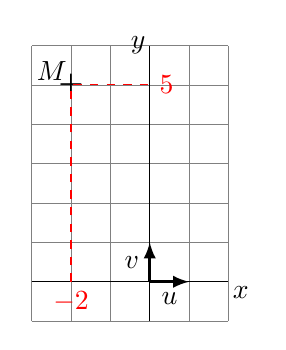
\begin{tikzpicture}[>=latex,scale=0.5]
            \draw[help lines] (-3,-1) grid (2,6);
            \draw[line width=0.5pt] (-3,0) -- (2,0) node[below right=-2pt] {$x$};
            \draw[->,line width=1pt] (0,0) -- (1,0) node[midway,below] {$\vect u$};
            \draw[line width=0.5pt] (0,-1) -- (0,6) node[left=-2pt] {$y$};
            \draw[->,line width=1pt] (0,0) -- (0,1) node[midway,left] {$\vect v$};
            \draw (-2,5) node {\textbf +} node[above left=-2pt] {$M$};
            \draw[red, dashed] (-2,0) node[below]{$-2$}|-(0,5) node[right] {$5$};
        \end{tikzpicture}
    \end{center}
\end{Exemple}

\begin{Defi}
    \begin{enumerate}
        \item Le point $M(x \pv y)$ est l'\iptb{image}\index{image d'un nombre complexe} du nombre complexe $z = x + y\I$.
        \item Le nombre complexe $z = x + y\I$ est l'\ipt{affixe} du point $M(x \pv y)$ et on note $z = aff(M)$ ou directement $M(z)$.
    \end{enumerate} 
\end{Defi}

\begin{Rmq}
    Le mot affixe est féminin : \textbf{une} affixe.
\end{Rmq}

Si $z = x + 0\I$ alors $z\in \R$ et on lui associe le point de coordonnées $(x \pv 0)$.\par
Si $z = 0 +y\I$ alors $z$ est un imaginaire pur et on lui associe le point de coordonnées $(0 \pv y)$.\par
On en déduit la propriété suivante :\medskip

\begin{Prop}
    \begin{enumerate}
        \item Un nombre réel a pour image un point situé sur l'axe des abscisses.
        \item Un imaginaire pur a pour image un point situé sur l'axe des ordonnées.
    \end{enumerate}
\end{Prop}

\begin{center}
    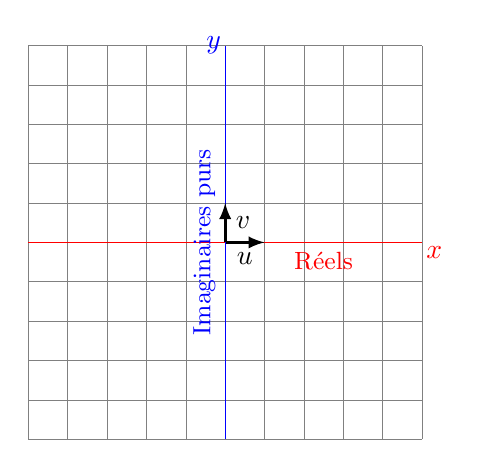
\begin{tikzpicture}[>=latex,scale=0.5]
        \draw[help lines] (-5,-5) grid (5,5);
        \draw[line width=0.5pt,red] (-5,0) -- (5,0) node[below right=-2pt] {$x$} node[below,pos=0.75] {\color{red}\small Réels};
        \draw[->,line width=1pt] (0,0) -- (1,0) node[midway,below] {$\vect u$};
        \draw[line width=0.5pt,blue] (0,-5) -- (0,5) node[left=-2pt] {$y$} node[midway,left] {\color{blue}\small\rotatebox{90}{Imaginaires purs}};
        \draw[->,line width=1pt] (0,0) -- (0,1) node[midway,right] {$\vect v$};
    \end{tikzpicture}
\end{center}

En seconde, il a été vu que le vecteur $\vect{OM}$ avait les mêmes coordonnées que le point $M$. En particulier, si $M$ a pour coordonnées $(x \pv y)$ alors $\vect{OM} = x\vect u + y \vect v$. On a alors la définition suivante :

\begin{Defi}
    \begin{enumerate}
        \item Le vecteur $\vect{OM}(x \pv y)$ est le \iptb{vecteur image}\index{vecteur image d'un nombre complexe} du nombre complexe $z = x + y\I$.
        \item Le nombre complexe $z = x + y\I$ est l'\ipt{affixe} du vecteur $\vect{OM}\binom{x}{y}$ et on note $z = aff\left(\vect{OM}\right)$ ou directement $\vect{OM}(z)$.
    \end{enumerate}
\end{Defi}

\begin{Exemple}
    Le point $A$ et le vecteur $\vect{AM}$ ont la même affixe : $z = 3 + \I$.
    \begin{center}
        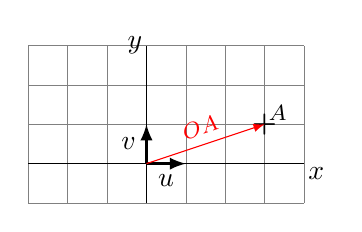
\begin{tikzpicture}[>=latex,scale=0.5]
            \draw[help lines] (-3,-1) grid (4,3);
            \draw[line width=0.5pt] (-3,0) -- (4,0) node[below right=-2pt] {$x$};
            \draw[->,line width=1pt] (0,0) -- (1,0) node[midway,below] {$\vect u$};
            \draw[line width=0.5pt] (0,-1) -- (0,3) node[left=-2pt] {$y$};
            \draw[->,line width=1pt] (0,0) -- (0,1) node[midway,left] {$\vect v$};
            \draw (3,1) node {\textbf +} node[above right=-2pt] {\footnotesize$A$};
            \draw[red, ->] (0,0)--(3,1) node[midway,above,sloped]{\footnotesize$\vect{OA}$};
        \end{tikzpicture}
    \end{center}
\end{Exemple}

\begin{Prop}
    On considère un point $M$ d'affixe $z$. Alors le point $N$ a pour affixe $\overline z$ si et seulement si $M$ et $N$ sont symétriques par rapport à l'axe des abscisses.
\end{Prop}

\begin{center}
    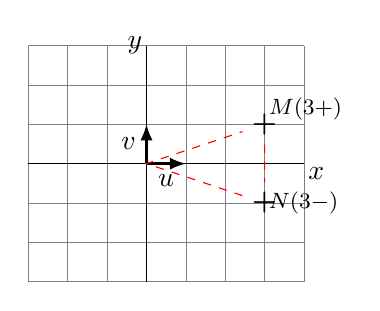
\begin{tikzpicture}[>=latex,scale=0.5]
        \draw[help lines] (-3,-3) grid (4,3);
        \draw[line width=0.5pt] (-3,0) -- (4,0) node[below right=-2pt] {$x$};
        \draw[->,line width=1pt] (0,0) -- (1,0) node[midway,below] {$\vect u$};
        \draw[line width=0.5pt] (0,-3) -- (0,3) node[left=-2pt] {$y$};
        \draw[->,line width=1pt] (0,0) -- (0,1) node[midway,left] {$\vect v$};
        \draw (3,1) node (M) {\textbf +} node[above right=-2pt] {\footnotesize$M(3+\I)$};
         \draw (3,-1) node (N) {\textbf +} node[right=-2pt] {\footnotesize$N(3-\I)$};
         \draw[dashed,red] (M)--(N)--(0,0)--(M);
    \end{tikzpicture}
\end{center}

\begin{Prop}
    On considère deux points $A$ et $B$ d'affixe respective $z_1$ et $z_2$.\par
    On place les points $C$ et $D$ tels que $\vect{OC} = \vect{OA} + \vect{OB}$ et $\vect{OD} = k.\vect{OA}$ ($k \in\R$).\par
    Alors l'affixe de $C$ est $z_3$ telle que :
    \[z_3 = z_1 + z_2\]
    et l'affixe de $D$ est $z_4$ telle que :
    \[z_4 = k.z_1.\]
\end{Prop}

\begin{center}
    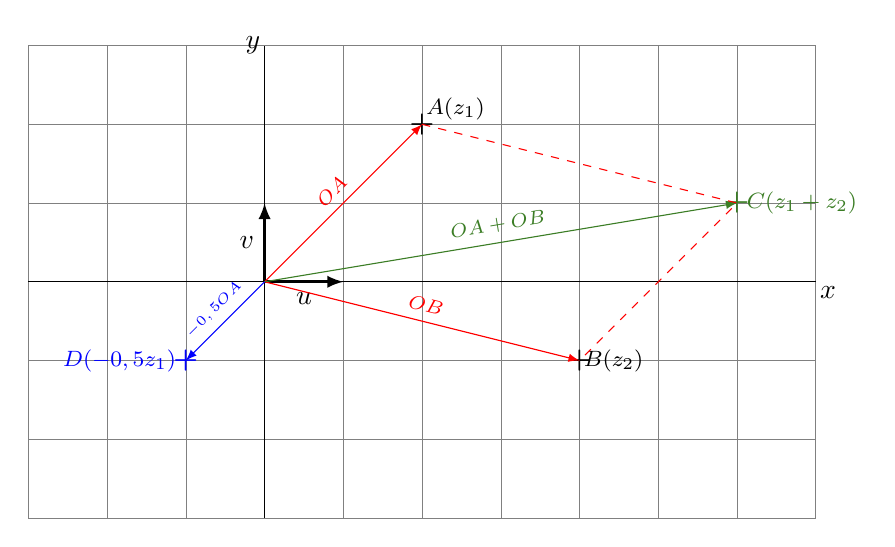
\begin{tikzpicture}[>=latex,scale=1]
        \draw[help lines] (-3,-3) grid (7,3);
        \draw[line width=0.5pt] (-3,0) -- (7,0) node[below right=-2pt] {$x$};
        \draw[->,line width=1pt] (0,0) -- (1,0) node[midway,below] {$\vect u$};
        \draw[line width=0.5pt] (0,-3) -- (0,3) node[left=-2pt] {$y$};
        \draw[->,line width=1pt] (0,0) -- (0,1) node[midway,left] {$\vect v$};
        \coordinate (A) at (2,2);
        \draw (A) node {\textbf +} node[above right=-2pt] {\footnotesize$A(z_1)$};
        \coordinate (B) at (4,-1);
         \draw (B) node {\textbf +} node[right=-2pt] {\footnotesize$B(z_2)$};
         \draw[red,->] (0,0)--(A) node[above,midway,sloped] {\scriptsize $\vect{OA}$};
         \draw[red,->] (0,0)--(B) node[above,midway,sloped] {\scriptsize $\vect{OB}$};
         \draw[color=OliveGreen,->] (0,0) -- (6,1) node {\textbf +} node[right] {\footnotesize $C(z_1 + z_2)$} node[above,midway,sloped] {\scriptsize $\vect{OA} + \vect{OB}$};
         \draw[color=blue,->] (0,0) -- (-1,-1) node {\textbf +} node[left] {\footnotesize $D(-0,5z_1)$} node[above,midway,sloped] {\tiny $-0,5\vect{OA}$};
         \draw[red,dashed] (A) -- (6,1) -- (B);
    \end{tikzpicture}
\end{center}
\end{document}
